\section{Valutazione delle performance}
La valutazione delle performance viene fatta per due motivi:
\begin{itemize}
    \item dal punto di vista dell'\textbf{utente} per ridurre il tempo di risposta. È nota anche come \textbf{tempo di esecuzione} o \textbf{latenza}. Definita come il tempo trascorso dall'inizio al completamento del compito o lavoro;

\item dal punto di vista del \textbf{sistema} per aumentare il \textbf{throughput}, ovvero la quantità totale di lavoro svolto in un dato intervallo di tempo, a volte chiamato \textbf{larghezza di banda}.

\end{itemize}

Lo speedup è definito come il rapporto tra il tempo di esecuzione di due programmi:
\begin{equation*}
	n=\frac{execTime_y}{execTime_x}
	=\frac{\frac{1}{\textsc{Performance}_y}}{\frac{1}{\textsc{Performance}_x}}=\frac{\textsc{Performance}_x}{\textsc{Performance}_y}
\end{equation*}
e misura il miglioramento delle prestazioni. \textbf{Nota:} il tempo di esecuzione è \textit{inversamente proporzionale} alle performance. Di solito $execTime_y$ viene sostituito dal tempo di esecuzione della versione sequenziale di un programma $P$ e $execTime_x$ con la sua versione parallelizzata.

Le misurazioni delle performance possono essere fatte a diversi livelli (considerando solo l'architettura hardware, una sua parte, o una parte di codice, o un intero programma, oppure tutto l'insieme) sfruttando funzionalità contenute in una \textbf{benchmark suite} (un insieme di tool di benchmark, come i \textbf{kernels} che sono piccoli pezzi di codice chiave presi da applicazioni reali, oppure i \textbf{toy programs} che contengono programmi, solitamente lunghi 100 linee di codice, che implementano algoritmi come la moltiplicazione tra matrici, il quicksort, e così via. Vi sono poi i \textbf{benchmark sintetici}, ovvero programmi ideati per simulare il comportamento delle applicazioni reali (come il Linpak, e il Dhrystone). La \textbf{SPEC} (Standard Performance Evaluation Corporation) è un consorzio senza scopo di lucro che stabilisce, mantiene e approva benchmark e strumenti standardizzati per valutare le prestazioni per la nuova generazione di sistemi informatici. SPEC sviluppa suite di benchmark e inoltre esamina e pubblica i risultati presentati dalle nostre organizzazioni membri e da altri licenziatari di benchmark.

Per comparare le performance di un componente hardware può essere consultata una \textbf{tabelle delle performance} dei modelli disponibili in commercio. Le informazioni più importanti riguardano i benchmark per completare un particolare task e il costo del componente hardware.

\subsection{Principio quantitativo} Per aumentare lo speedup è necessario concentrare le energie sul codice che viene eseguito più frequentemente, piuttosto che quello eseguito più raramente.

Un importante riferimento a tal proposito, è la \textbf{legge di Amdahl}.
\newpage
\paragraph{Legge di Amdahl.}
\begin{mdframed}
    \textit{"Il miglioramento delle prestazioni di un sistema che si può ottenere ottimizzando una certa parte del sistema è limitato dalla frazione di tempo in cui tale parte è effettivamente utilizzata"}.
\end{mdframed}
Di seguito con $f_i \le 1$ (\textit{"fraction improved"}) viene indicata la frazione del tempo di esecuzione della macchina originale (o del codice originale) che può essere modificata per trarre vantaggio dalle migliorie, mentre con $s_i \ge 1$ (\textit{"speedup improved"}) viene indicato il miglioramento ottenuto da un una modalità di esecuzione più veloce.
\begin{align}
    e_n &= e_o \cdot \left((1-f_i) + \frac{f_i}{s_i} \right) \label{eqn:execution-time-new} \\
    s_g &= \frac{e_o}{e_n}= \frac{1}{(1-f_i)+ \frac{f_i}{s_i}}\label{eqn:speedup-global}
\end{align}
Se un miglioramento può essere usato solo per una frazione dell'intero task:
\begin{equation}
    s_g = \frac{1}{(1-f_i)+\frac{f_i}{s_i}} \fcolorbox{red}{white}{$\le \frac{1}{(1-f_i)}$} \label{eqn:speedup-global-with-limit}
\end{equation}
\begin{eqnarray}
    \begin{tblr}{|c|c|}
    \hline
       e_n & \text{execution time new}
       \\
       \hline
       e_o & \text{execution time old}
       \\
       \hline
       f_i & \text{fraction improved}
       \\
       \hline
       s_i & \text{speedup improved}
       \\
       \hline
       s_g & \text{speedup global}
       \\
       \hline
    \end{tblr}
\end{eqnarray}

Lo \textbf{speedup globale} $s_g$ è uguale a $ \frac{1}{(1-f_i)+\frac{f_i}{s_i}}$ dove $1-f_i$ è la frazione non parallelizzabile, $f_i$ è la frazione parallelizzabile e $s_i$ è lo speedup che si ottiene dalla porzione parallelizzabile di codice. Lo speedup globale massimo, nel riquadro rosso (equazione \ref{eqn:speedup-global-with-limit}) si ottiene facendo tendere la $s_i$ all'infinito: \[\lim_{s_i \to \infty}{\frac{f_i}{s_i}} = 0\]
\begin{exercise}
	Si consideri un miglioramento di 10 volte più veloce della macchina originale (o del codice) ma che può essere applicato solo per il 40\% del tempo. Qual'è il guadagno totale?
\end{exercise}
\begin{solution}
	Traendo i dati dal problema, si ottiene che lo $s_i = 10$ e che $f_i = 40\% = 0,4$. Sostituendo alla formula \ref{eqn:speedup-global} si ottiene
	\begin{equation*}
		s_g = \frac{1}{(1-0.4)+\frac{0.4}{10}} = \frac{1}{0.6+0.04} = \frac{1}{0.64} = \frac{100}{64} = 1.56
	\end{equation*}

	Lo speedup ottenuto è di 1.56.
\end{solution}

\begin{exercise}
	Si consideri una CPU che è stata aggiornata per avere i seguenti cambiamenti:
	\begin{enumerate}
		\item aumentare la velocità di un fattore pari a 5 senza interessare le performance del sistema I/O;
		\item il costo è 5 volte superiore al precedente;
		\item la CPU può essere utilizzata per il 50\% del tempo totale, mentre il rimanente viene impiegato per operazioni di I/O;
		\item il costo della CPU è $\frac{1}{3}$ del costo della macchina.
	\end{enumerate}
	Questo investimento, è conveniente?
\end{exercise}
\begin{solution}
	Lo $s_i = 5$, la $f_i = 50\% = 0.5$. Lo speedup globale è:
	\begin{equation*}
		s_g = \frac{1}{(1-0.5)+\frac{0.5}{5}}=\frac{1}{0.5+0.1} = \frac{10}{6} = 1.67
	\end{equation*}
	il costo è aumentato di:
	\begin{equation*}
		c = 1 \cdot \frac{2}{3} + 5 \cdot \frac{1}{3} =\frac{7}{3} = 2.33
	\end{equation*}
	Dato che il costo è superiore al rendimento ottenuto $ c = 2.33 >  s_g = 1.67 $ non è conveniente fare l'aggiornamento del processore.
\end{solution}

\begin{exercise}
	Si vuole riscrivere un programma su un'architettura MIMD con 100 processori. L'obbiettivo è di ridurre il tempo di esecuzione di 80 volte rispetto a quello precedente su un'architettura SISD. Qual'è la frazione del programma originale che può restare sequenziale?
\end{exercise}
\begin{solution}
	L'impostazione del problema è diversa dai precedenti. Il tempo di esecuzione della soluzione parallela è 80 volte più veloce di quella sequenziale. Si può osservare che il tempo totale è dato dalla somma del tempo di esecuzione della parte sequenziale e di quella parallela.
	\begin{align*}
		T&=\frac{T_{\textsc{sisd\textsubscript{\textsc{par}}}}}{\#\textsc{processori}}+\textsc{T\textsubscript{SISD}\textsubscript{\textsc{nonpar}}}\\
		&=\frac{T\textsubscript{\textsc{sisd}}\cdot \%\textsc{par}}{\#\textsc{processori}}+T_\textsc{sisd}\cdot\underbrace{ (1-\% par) }_{\%\textsc{nonpar}}
	\end{align*}
	La percentuale parallelizzabile è dell' $80\%$ rispetto al tempo iniziale ($T_\textsc{SISD}$).  Il numero di processori è $100$. Per semplicità si imposta ad $x=\% par$, ovvero la percentuale cercata.
	Sostituendo i dati nella formula:
	\begin{align*}
		\frac{\cancel{T_\textsc{sisd}}}{80}&=T_{\cancel{\textsc{sisd}}}\cdot \left(\frac{x}{100}+\underbrace{(1-x)}_{\textsc{\% nonpar}}\right)\\
		\frac{1}{80} &=  \frac{x}{100} + (1-x)\implies \frac{x+100-100\, x}{100}=\frac{1}{80}
		 \\ &\implies x = \left(\frac{5}{4}-100\right)\cdot\frac{1}{-99}\implies x = \frac{-395}{4}\cdot \frac{1}{-99}=0.997\\ &\implies x = 99.7\%
	\end{align*}
\end{solution}

\begin{exercise}
	Sapendo che il calcolo parallelo è 20 volte più veloce rispetto all'originale (sequenziale), calcolare:
	\begin{itemize}
		\item  la percentuale di parallelismo è la porzione di tempo impiegata utilizzando la modalità di esecuzione SIMD.
		\item Disegna un grafico per rappresentare il miglioramento delle prestazioni come percentuale del calcolo eseguito in modalità SIMD.
		\item  Quale percentuale di parallelismo è necessaria per ottenere un miglioramento delle prestazioni pari a 2? Quale per raggiungere la metà del miglioramento massimo?
	\end{itemize}
\end{exercise}
\begin{solution}
	Lo speedup che si ottiene è il seguente. Si pone $x=\% par$
	\begin{align*}
		\textsc{speedup} = \frac{1}{(1-x)+\frac{x}{\text{speedup par.}}} = \frac{1}{(1-x)+\frac{x}{20}} = \frac{20}{20-19 \, x}
	\end{align*}
	Il grafico è il seguente.
	\begin{figure}[ht]
		\centering
		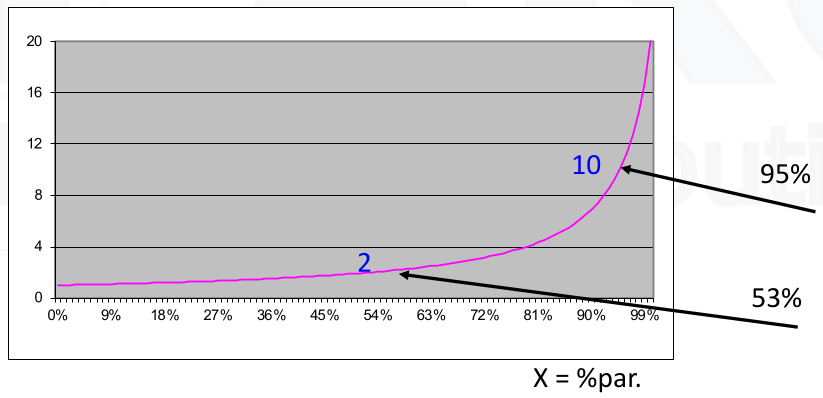
\includegraphics[width=0.7\linewidth]{img/graph-ex4}
		\caption{grafico dello speedup.}
		\label{fig:graph-ex4}
	\end{figure}
\end{solution}
Si consideri ora lo stesso esercizio ma con questi dati.
\begin{exercise}
	La percentuale di parallelismo raggiungibile è del 70\%. Ci sono due alternative.
	\begin{enumerate}
		\item Raddoppiare la velocità della modalità SIMD (è molto costoso)
		\item Aumentare la percentuale di parallelismo concentrandosi sul compilatore.
	\end{enumerate}
	Quale \textbf{aumento} della percentuale di parallelismo è necessario per ottenere lo stesso guadagno di prestazioni?
\end{exercise}
\begin{solution}
	Lo speedup originale si ottiene facendo
	\begin{equation*}
		\textsc{speedup orig}[20 \cdot 70 \%] = \frac{1}{(1-0.7)+\frac{0.7}{20}} = \frac{20}{20-14+0.7}=2.9851
	\end{equation*}
	Raddoppiando la velocità della modalità SIMD
	\begin{equation*}
		\textsc{speedup hw}[20 \cdot 70\%] = \frac{1}{(1-0.7)+\frac{0.7}{40}}=\frac{40}{40-28+0.7}=3.1496
	\end{equation*}
	Lo speedup adottando il compilatore è ovviamente parametrico, perché ci si sta chiedendo quale sia la percentuale necessaria per ottenere lo stesso guadagno di prestazioni, ed è il seguente.
	\begin{equation*}
		\textsc{speedup compiler}[20\cdot x\%] = \frac{1}{(1-x)+\frac{x}{20}}=\frac{20}{20-19\, x}
	\end{equation*}
	Si pone dunque
	\[\textsc{speedup compiler}= \textsc{speedup hw}\]
	ovvero
	\begin{equation*}
		\frac{20}{20-19\, x} = 3.1496 \implies x = 0.7184
	\end{equation*}
	Dunque è sufficiente una parallelizzazione del 71.84\%.
\end{solution}
\begin{exercise}
	Si consideri un'architettura basata su cache. La memoria cache è 5 volte più veloce della memoria principale. La cache è usata per il 90\% del tempo. Ci si chiede quale sia lo speedup con e senza cache.
\end{exercise}
\begin{solution}
	Lo speedup è il seguente.
	\begin{equation*}
		\textsc{speedup} = \frac{1}{(1-x)+\frac{x}{\textsc{speedup con cache}}} = \frac{1}{(1-0.9)+\frac{0.9}{5}}=\frac{1}{0.28}\approx 3.6
	\end{equation*}
	Si conclude che l'architettura basata su cache è più veloce di 3.6 volte la velocità della stessa architettura senza cache.
\end{solution}
%%%%%%%%%%%%%%%%%%%%%%%%%%%%%%%%%%%%%%%%%%%%%%%%%%%%%%%%%%%%%%%%%%%%%%%%

\subsection{Tempo di esecuzione} Il tempo di esecuzione viene usato per misurare le performance di un computer: l'architettura che esegue la stessa quantità di lavoro in meno tempo è la più veloce. Il \textbf{tempo di risposta} rappresenta la latenza per completare un task e include accessi al disco, gli accessi alla memoria e le operazioni di input/output. Il \textbf{CPU time} ovvero il tempo impiegato per svolgere operazioni di CPU (cicli di clock per eseguire il codice interessato, per operazioni di sistema -- ad esempio per la stampa a video -- mentre non è considerato CPU time il tempo speso per attendere dati o istruzioni accedendo in memoria perché è un tempo di attesa. 
Il CPU time è calcolato come segue:
\begin{align*}
\text{CPU\textsubscript{\textsc{time}}} &= \text{Cicli di clock della CPU per una task} * \text{tempo di un ciclo di clock}\\
&= \frac{\text{Cicli di clock della CPU per una task}}{\text{Frequenza di clock}}
\end{align*}

I Cicli di clock medi per istruzione (CPI) medi vengono calcolati come segue:
\begin{align*}
\text{CPI} &= \frac{\text{Cicli di clock della CPU per una task}}{\text{Numero di istruzioni}}\\
\text{CPU\textsubscript{\textsc{time}}} &= \text{N di istruzioni} * \text{CPI} * \text{durata di un ciclo di clock}\\
&= \frac{\text{N di istruzioni} * \text{CPI}}{\text{Frequenza di clock}}\\
T\textsubscript{\textsc{{cpu}}} &= \text{CI}* \text{CPI} * T\textsubscript{\textsc{clock}} = \frac{\text{CI} * \text{CPI}}{f\textsubscript{\textsc{{clock}}}}
\end{align*}

La relazione tra le varie metriche è visibile di seguito:
\begin{align*}
    \frac{\text{istruzioni}}{\text{task}} * \frac{\text{cicli di clock}}{\text{istruzione}} * \frac{\text{secondi}}{\text{cicli di clock}}= \frac{\text{secondi}}{\text{task}} = \text{CPU time}
\end{align*}

Il tempo di CPU dipende da 3 parametri:
\begin{itemize}
    \item \textbf{Ciclo di clock (o frequenza)}: dipende dalla tecnologia, quindi l'unico modo per migliorare questo parametro consiste nel sostituire l'architettura.
    \item \textbf{CPI}: è il numero di cicli di clock medio per istruzione. Dipende dall'organizzazione dell'architettura e dall'istruction set architecture (ISA), che è l'insieme delle istruzioni che vengono gestite dall'architettura; se queste sono complesse, richiedono generalmente più cicli di clock.
    \item \textbf{Numero di istruzioni}: il numero di istruzioni usate da un programma dipende dall'instruction set architecture e dalla tecnologia del compilatore. Un buon compilatore permette idealmente di avere un codice finale con meno istruzioni (ovviamente un fattore importante rimane la capacità del programmatore). Questo parametro è quello in cui è più fattibile intervenire.
\end{itemize}

Il numero totale di cicli di clock per una task si calcola come segue:
\begin{align*}
    \text{Cicli di clock della CPU} = \sum^n_{i=1} (CPI_i * I_i)
\end{align*}
dove:
\begin{itemize}
    \item $I_i$ rappresenta il numero di volte in cui l'istruzione $I$ è stata eseguita in una task;
    \item $CPI_i$ rappresenta il numero medio di cicli di clock spesi per una generica istruzione.
\end{itemize}

Date queste misure, il CPU time può essere riscritto come:
\begin{align*}
    T_{CPU} = \sum^n_{i = 1} (CPI_i * I_i) * T_{CLOCK}
\end{align*}

\begin{exercise}
	Si supponga di avere effettuato le seguenti  misurazioni.
	\begin{itemize}
		\item Frequenza delle operazioni in virgola mobile (incluse le FPSQR) = 25\%
		\item CPI medio delle operazioni in virgola mobile = 4.0
		\item Frequenza delle operazioni FPSQR (radice quadrata in virgola mobile) = 2\%
		\item CPI delle operazioni FPSQR = 20.0
	\end{itemize}
	Ci sono due possibilità:
	\begin{enumerate}
		\item Decrementare la CPI del FPSQR a 2
		\item Decrementare il CPI medio di tutte le operazioni FP (floating point) di 2.5
	\end{enumerate}
	Comparare le due alternative in termini di performance complessive.
\end{exercise}
\begin{solution}
	Si ricava il CPI originale
	\begin{equation*}
		\textsc{cpi}_{\textsc{orig}}=(0.25\cdot 4)+(0.75 \cdot 1.33)=2.00
	\end{equation*}
	Si può calcolare il CPI per l'FPSQR migliorato, sottraendo i cicli risparmiati dal CPI originale:
	\begin{align*}
		\textsc{cpi}_1 &= \textsc{cpi}_{\textsc{orig}}-2\% \cdot \left(\textsc{cpi}_{\textsc{old\_fspqr}}-\textsc{cpi}_\textsc{new\_fspq\_only}\right)\\&=2.00-2\%\cdot(20-2)=1.64
	\end{align*}
	È possibile calcolare il CPI per il miglioramento di tutte le istruzioni FP e allo stesso modo sommando i CPI delle istruzioni FP e non FP. Utilizzando quest'ultimo metodo si ottiene:
	\begin{equation*}
		\textsc{cpi}_2 = \left(75\% \cdot 1.33\right)+(25\% \cdot 2.5) = 1.625
	\end{equation*}
	Dato che il CPI del miglioramento complessivo delle istruzioni FP è leggermente più basso, le sue prestazioni saranno leggermente migliori. Nello specifico, il miglioramento delle prestazioni complessive delle istruzioni FP è:
	\begin{align*}
			\textsc{speedup}_2 = \frac{\textsc{cpu\textsubscript{time\textsubscript{orig}}}}{\textsc{cpu\textsubscript{time\textsubscript{2}}}}= \frac{\textsc{ic}\cdot \textsc{clock\textsubscript{cycle}}\cdot \textsc{cpi}\textsubscript{\textsc{orig}}}{\textsc{ic}\cdot \textsc{clock\textsubscript{cycle}}\cdot \textsc{cpi}\textsubscript{\textsc{2}}}=\frac{\textsc{cpi\textsubscript{orig}}}{\textsc{cpi\textsubscript{2}}}=\frac{2.00}{1.625}=1.23
	\end{align*}
\end{solution}
\begin{exercise}
	L'architettura inizialmente dispone solo di istruzioni di caricamento e memorizzazione per accedere alla memoria. Tutte le altre operazioni lavorano nei registri (architettura L/S). Il riassunto delle istruzioni è riportato nella tabella.
	\begin{table}[ht]
		\centering
		\begin{tabular}{|l|c|c|}
			\hline
			& \textbf{Frequenza}&\textbf{Cicli di clock}
			\\\hline
			ALU & 43\% & 1
			\\\hline
			Load & 21\% & 2
			\\\hline
			Store & 12\% & 2
			\\\hline
			Branch & 24\% & 2
			\\\hline
		\end{tabular}
	\end{table}
	Si supponga che il 25\% delle operazioni dell'ALU utilizzi un operando specificamente caricato, che non è più utile per le operazioni successive. Viene proposto di aggiornare il set di istruzioni avendo uno degli operandi di origine in memoria. Queste nuove operazioni reg-mem hanno un numero di cicli di clock pari a 2 e richiedono 3 cicli di clock per i salti, senza modificare il periodo del ciclo di clock. Questa modifica può migliorare le prestazioni della CPU?
\end{exercise}
\begin{solution}
	Si ottiene $\textsc{cpi\textsubscript{old}}$
	\begin{equation*}
		\textsc{cpi\textsubscript{old}} = 0.43 \cdot 1 + 0.21 \cdot 2 + 0.12 \cdot 2 + 0.24 \cdot 2 = 1.57
	\end{equation*}
	Il tempo di $\textsc{cpi}\textsubscript{old}$ si ottiene come:
	\begin{equation*}
		\textsc{t\textsubscript{cpu\textsubscript{old}}} = \textsc{ci\textsubscript{old}} \cdot1.57 \cdot \textsc{t\textsubscript{clock\textsubscript{old}}}
	\end{equation*}
	il $\textsc{cpi}\textsubscript{new}$ è:
	\begin{equation*}
		\textsc{cpi\textsubscript{new}} = \frac{\splitfrac{(0.43-(0.25 \cdot 0.43))\cdot 1+(0.21-(0.25\cdot 0.43))\cdot 2+}{ +(0.25\cdot 0.43)\cdot 2+ 0.12 \cdot 2 + 0.24 \cdot 3}}{1-(0.25 \cdot 0.43)}
	\end{equation*}
	Si ricava il$\textsc{t\textsubscript{cpu\textsubscript{new}}}$:
	\begin{equation*}
		\textsc{t\textsubscript{cpu\textsubscript{new}}}=(0.893\cdot \textsc{ci\textsubscript{old}})\cdot(1.908 \cdot \textsc{t\textsubscript{clock\textsubscript{old}}})=1.703 \cdot \textsc{ci\textsubscript{old}} \cdot \textsc{t\textsubscript{clock\textsubscript{old}}}
	\end{equation*}
	L'introduzione delle istruzioni reg-mem non compensa l'aumento del tempo di esecuzione dei salti.
\end{solution}
\subsection{MIPS e GIPS}
Con le sigle MIPS e GIPS si intendono rispettivamente milioni di microistruzioni per secondo e miliardi di microistruzioni per secondo, dove:
\begin{align*}
    MIPS &= \frac{\text{N di istruzioni}}{\text{Tempo di esecuzione} * 10^6}\\
    &= \frac{\text{frequenza di clock}}{CPI * 10^6}
\end{align*}

Il tempo di esecuzione diventa:
\begin{align*}
    \text{Tempo di esecuzione} = \frac{\text{N di istruzioni}}{MIPS * 10^6}
\end{align*}
\
Poiché MIPS rappresenta la frequenza di operazioni per unità di tempo, le performance per la macchina più veloce cha ha alti valori MIPS può essere specificata come l'inversa del tempo di esecuzione. Il vantaggio del MIPS è che è semplice da capire: le macchine più veloci hanno valori MIPS più alti. 

La metrica MIPS presenta comunque una serie di problematiche:
\begin{itemize}
    \item Il valore dipende dall'instruction set, quindi è difficile da comparare con macchine che hanno diversi instruction set;
    \item Varia in base al programma considerato;
    \item Varia in modo inversamente proporzionale alla performance.
\end{itemize}

La limitazione principale di questa misura è che non considera il tipo di istruzioni eseguite. Ad esempio, le operazioni su interi sono generalmente più







Se ci interessa misurare nello specifico le performance relative alle operazioni floating-point possiamo utilizzare la metrica GFLOPS, che sta per \textbf{billion of FP instructions per second} (dove FP indica le operazioni floating-point):
\begin{align*}
    GFLOPS = \frac{\text{N di \textbf{operazioni} FP in un programma}}{\text{Tempo di esecuzione} * 10^9}
\end{align*}

Ovviamente questa metrica non può essere usata in contesti diversi da quelli legati alle operazioni FP. Essendo basata su operazioni piuttosto che istruzioni, i FLOPS sono concepiti per essere un buon metodo di confronto tra le varie architetture. L'ipotesi è che stesso programma, lanciato su differenti architetture, esegue un diverso numero di istruzioni, ma lo stesso numero di operazioni floating-point. Le operazioni FP non sono considerate tra diverse architetture; il GFLOPS cambia cambiando il rapporto tra le operazioni intere e FP oppure cambiando il mix di operazioni FP veloci e lente.

Il \textbf{Normalized GFLOPS} prevede di associare un bias, con funzione di peso, ad ogni operazione FP, come mostrato in figura \ref{fig:normalized-gflops}.
\begin{figure}[th]
	\centering
	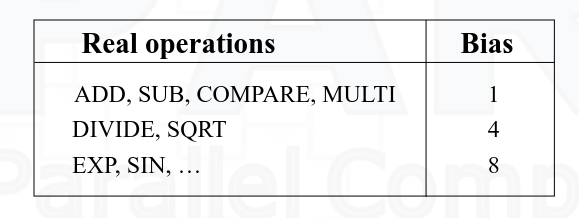
\includegraphics[width=0.7\linewidth]{img/normalized-gflops.png}
	\caption{Esempio di bias per operazioni FP.}
	\label{fig:normalized-gflops}
\end{figure}

Un frammento di codice con operazioni un'operazione ADD, una DIVIDE e una SIN, si calcola avere 12 operazioni FP normalizzate.
\newpage
\begin{exercise}
	Il programma Spice viene eseguito su una DECstation 3100 in 0,094 secondi. Il numero di operazioni in virgola mobile eseguite dal programma è riportato nella tabella.
	\begin{table}[ht]
		\centering
		\scriptsize
		\begin{tabular}{|l|r|}
			\hline
			addD & 25,999,440
			\\\hline
			subD & 18,266,439
			\\\hline
			mulD & 33,880,810
			\\\hline
			divD & 15,682,333
			\\\hline
			compareD & 9,745,930
			\\\hline
			negD & 2,617,846
			\\\hline
			absD & 2,195,930
			\\\hline
			convertD & 1,581,450
			\\\hline
			\textbf{totale} & \textbf{109,970,178}
			\\\hline
		\end{tabular}
	\end{table}
	Calcolare:
	\begin{itemize}
		\item I GFLOPS del programma.
		\item I GFLOPS normalizzati.
	\end{itemize}
\end{exercise}
\begin{solution}
	\begin{align*}
		\textsc{ci\textsubscript{ott}} &= \textsc{ci\textsubscript{non ott}}\cdot \left[(1-0.3)\cdot \left(1-\frac{1}{3}\right)\right]=0.9 \cdot \textsc{ci\textsubscript{non ott}}\\
		\textsc{ci\textsubscript{ott}} &= \textsc{cpi\textsubscript{non ott}}=1\\
		\textsc{t\textsubscript{\textsc{clock\textsubscript{ott}}}} &= 1.05 \cdot \textsc{t\textsubscript{\textsc{clock\textsubscript{non ott}}}}\\
		\textsc{t\textsubscript{cpu\textsubscript{ott}}} &= 0.9 \cdot \textsc{ci\textsubscript{non ott}} \cdot \textsc{cpi\textsubscript{\textsc{non ott}}}\cdot\textsc{t\textsubscript{clock\textsubscript{non ott}}}\\
		&=0.945 \cdot \textsc{ci\textsubscript{non ott}}\cdot \textsc{cpi\textsubscript{non ott}}\cdot \textsc{t\textsubscript{clock\textsubscript{non ott}}}\\
		&= 0.945 \cdot \textsc{t\textsubscript{cpu\textsubscript{non ott}}}
	\end{align*}
\end{solution}














